% Template for PLoS
% Version 3.8 Apr 2026
% Adapted for: "A Four-Dimension Pre-Modeling Audit Protocol for
% Educational Prediction Benchmarks: Evidence from Seven Public Datasets"
% Yan Ma & Lizhuo Zhang

\documentclass[10pt,letterpaper]{article}
\usepackage[top=0.85in,left=2.75in,footskip=0.75in]{geometry}

% amsmath and amssymb packages, useful for mathematical formulas and symbols
\usepackage{amsmath,amssymb}

% Use adjustwidth environment to exceed column width (see example table in text)
\usepackage{changepage}

% textcomp package and marvosym package for additional characters
\usepackage{textcomp,marvosym}

% cite package, to clean up citations in the main text. Do not remove.
% NOTE: we use natbib [numbers] so that \citep and \citet work throughout the body.
\usepackage[numbers,sort&compress]{natbib}

% Use nameref to cite supporting information files (see Supporting Information section for more info)
\usepackage{nameref,hyperref}
\hypersetup{colorlinks=false,pdfborder={0 0 0}}

% line numbers
\usepackage[right]{lineno}
\usepackage{indentfirst}
\usepackage{needspace}
\usepackage{placeins}

% ligatures disabled
\usepackage{microtype}

% color can be used to apply background shading to table cells only
\usepackage[table]{xcolor}

% array package and thick rules for tables
\usepackage{array}
\usepackage{booktabs}
\usepackage{multirow}
\usepackage{graphicx}
\usepackage{float}

% create "+" rule type for thick vertical lines
\newcolumntype{+}{!{\vrule width 2pt}}

% create \thickcline for thick horizontal lines of variable length
\newlength\savedwidth
\newcommand\thickcline[1]{%
  \noalign{\global\savedwidth\arrayrulewidth\global\arrayrulewidth 2pt}%
  \cline{#1}%
  \noalign{\vskip\arrayrulewidth}%
  \noalign{\global\arrayrulewidth\savedwidth}%
}

% \thickhline command for thick horizontal lines that span the table
\newcommand\thickhline{\noalign{\global\savedwidth\arrayrulewidth\global\arrayrulewidth 2pt}%
\hline
\noalign{\global\arrayrulewidth\savedwidth}}

% Text layout
\raggedright
\setlength{\parindent}{0.5cm}
\textwidth 5.25in
\textheight 8.75in

% Bold the 'Fig #' in the caption and separate it from the title/caption with a period
\usepackage[aboveskip=1pt,labelfont=bf,labelsep=period,justification=raggedright,singlelinecheck=off]{caption}
\renewcommand{\figurename}{Fig}

% Please use the included plos2025.bst as your BibTeX style
\bibliographystyle{plos2025}

% Remove brackets from numbering in List of References
\makeatletter
\renewcommand{\@biblabel}[1]{\quad#1.}
\makeatother

% Header and Footer with logo
\usepackage{lastpage,fancyhdr}
\usepackage{epstopdf}
\pagestyle{fancy}
\fancyhf{}
\rfoot{\thepage/\pageref{LastPage}}
\renewcommand{\headrulewidth}{0pt}
\renewcommand{\footrule}{\hrule height 2pt \vspace{2mm}}
\fancyheadoffset[L]{2.25in}
\fancyfootoffset[L]{2.25in}
\lfoot{\today}


\begin{document}
\vspace*{0.2in}

% ── Title & Author block ──────────────────────────────────────────────────────
\begin{flushleft}
{\Large
\textbf{A Four-Dimension Pre-Modeling Audit Protocol for Educational Prediction
Benchmarks: Evidence from Seven Public Datasets}
}
\newline
\\
Yan Ma\textsuperscript{1,3},
Lizhuo Zhang\textsuperscript{2,*}
\\
\bigskip
\textbf{1} School of Education, Hunan Agricultural University,
  Changsha 410128, China \\
\textbf{2} School of Information and Intelligence, Hunan Agricultural University,
  Changsha 410128, China \\
\textbf{3} School of Foreign Studies, Changsha University of Science and Technology,
  Changsha 410114, China \\
\bigskip

* \textbf{Corresponding author}\\
E-mail: zhanglizhuo@hunau.edu.cn
\end{flushleft}

% ── Abstract (≤ 300 words) ────────────────────────────────────────────────────
\section*{Abstract}
Predictive models in education increasingly inform high-stakes decisions, yet the
datasets underlying these models are rarely stress-tested before modeling begins.
This paper proposes a four-dimension pre-modeling audit protocol that checks
educational prediction benchmarks along baseline gap, split instability, null
separation, and metadata adequacy---the last operationalized as group-aware
holdout. Applying the protocol to seven public datasets ($N=145$ to $32{,}593$),
the results show that five of seven datasets fail metadata adequacy: four fail
linear-model group-aware holdout (two show model-invariant confounding with
$R^2$ collapsing to negative values for all model types, two show remediable
linear-specific overfitting that regularized and ensemble models can partially
alleviate), and one (MM-TBA) cannot be tested because grouping metadata is
unavailable. A model-complexity
ablation confirms that data-level fragility is algorithm-invariant: ensemble models
amplify instability on fragile data ($I \approx 4.6$ vs.\ $2.2$) while yielding
genuine gains only on structurally sound data. A classification-metric sensitivity
check confirms that audit profiles are robust to metric choice. The paper proposes
operational decision criteria and a reusable four-step audit checklist. The
protocol and all analysis code are publicly available.

\clearpage
\newgeometry{top=0.85in,left=1in,right=1in,footskip=0.75in}
\linenumbers

% ── Body ─────────────────────────────────────────────────────────────────────
\section{Introduction}

Educational AI increasingly uses predictive models to inform teaching evaluation, student intervention, and institutional policy. Yet many reported gains remain hard to interpret because dataset integrity is rarely audited before modeling. In computer vision and NLP, benchmark-audit studies have become routine \citep{Northcutt2021,Recht2019,Bouthillier2021}, but no comparable audit protocol exists for the educational prediction domain---despite the fact that educational decisions are often higher-stakes and educational datasets more vulnerable to group-level confounding than the image-classification benchmarks where most audit work has been conducted.

This gap is consequential. Educational datasets typically contain nested group structure---students within classrooms, classrooms within schools, schools within districts---that creates confounding risks absent from standard ML benchmarks. If teacher identity, school culture, or cohort composition are under-specified, a model can learn contextual shortcuts rather than generalizable pedagogical signal. Under those conditions, high correlation is not evidence of instructional quality; it may reflect unresolved group-level confounding, label noise, or non-independent partitions. The growing use of LLM-derived scoring in educational assessment introduces additional risk: if both features and targets originate from the same automated pipeline, apparent predictive performance may reflect shared artifacts rather than pedagogical signal.

The present study addresses this gap by proposing and validating a structured four-dimension pre-modeling audit protocol for educational prediction benchmarks. The protocol checks each dataset along baseline gap (does the model beat a trivial reference?), split instability (is the conclusion robust to random-seed variation?), null separation (can the signal be distinguished from permuted labels?), and metadata adequacy (does performance survive group-aware holdout?). In the terminology of meta-science \citep{Ioannidis2005}, the protocol asks not "how well can we predict?" but "should we be predicting at all, given the data we have?" The individual diagnostic tools---repeated resampling, permutation tests, group holdout---are well established; the contribution is their systematic integration into a reusable audit protocol and its empirical validation across seven public educational datasets spanning $N = 145$ to $32{,}593$ (see Table 1).

The study makes three contributions. (1) It proposes a reusable four-dimension audit protocol with operational thresholds that educational AI practitioners can apply before investing in complex modeling. (2) The seven-dataset validation reveals that five of seven educational benchmarks fail metadata adequacy: four fail group-aware holdout under linear models (two with model-invariant confounding, two with remediable linear-specific overfitting), and one cannot be tested because grouping metadata is unavailable. This failure rate is far higher than would be expected if current benchmarking practice were adequate, suggesting group-aware validation should become routine. (3) The model-complexity ablation demonstrates that data-level fragility is algorithm-invariant: escalating from linear baselines to ensemble methods amplifies instability on fragile datasets. The protocol adds an empirical stress-test layer to documentation-oriented work such as Datasheets for Datasets \citep{Gebru2021} and data-cascade critiques \citep{Sambasivan2021}.

\section{Related Work}

The present study sits at the intersection of four adjacent literatures: benchmark auditing in machine learning, educational data mining and learning analytics, educational measurement theory, and dataset documentation or quality assurance. Reviewing these strands together clarifies why a pre-modeling audit protocol is needed in educational prediction and what is substantively new about the present paper.

\textbf{(1) Benchmark auditing in machine learning.} The recognition that benchmark conclusions can be fragile predates the current study. Northcutt et al.~\citep{Northcutt2021} showed that pervasive label errors in widely used test sets destabilize model rankings. Recht et al.~\citep{Recht2019} demonstrated that classifiers trained on ImageNet lose accuracy when evaluated on independently collected test sets matching the original distribution. Bouthillier et al.~\citep{Bouthillier2021} quantified how random-seed and split variation inflates apparent method differences, recommending that benchmark papers report variance across admissible protocol choices. These findings motivate the split-instability and null-separation dimensions of the present audit. However, nearly all existing audit work targets computer-vision or NLP benchmarks; comparable systematic audits of educational prediction datasets remain scarce.

\textbf{(2) Educational data mining and learning analytics.} The EDM and learning analytics communities have developed a large body of work on predicting student outcomes \citep{Romero2020}. Baker et al.~\citep{Baker2014} surveyed EDM methods; Gardner et al.~\citep{Gardner2019} examined feature engineering practices in student-success prediction. Several studies have noted the importance of cross-institutional generalization \citep{Chejara2023,Chejara2024}, but the standard practice remains iid train-test evaluation without explicit group-aware holdout. Methodological audits of the datasets themselves---as opposed to the models trained on them---are rare.

\textbf{(3) Educational measurement theory.} The split-instability dimension of the audit connects to longstanding concerns in educational measurement. Generalizability Theory (G-theory; Brennan~\citep{Brennan2001}) decomposes score variance into facets (persons, raters, occasions, items) and estimates the generalizability coefficient $G = \sigma^2_p / (\sigma^2_p + \sigma^2_{\text{error}})$. The instability ratio $I$ used here serves an analogous function: when $I \geq 1$, the between-split variance exceeds the mean signal, indicating that the "score" (model performance) is not generalizable across the "facet" of train-test partitioning. The metadata-adequacy dimension parallels the validity-argument framework \citep{Messick1995,Kane2006}, which requires that score interpretations be supported by evidence spanning content, substantive, structural, generalizability, external, and consequential aspects. A dataset that fails group-aware holdout lacks generalizability evidence in the Messick sense, regardless of its iid performance. These connections ground the audit protocol in a mature psychometric tradition that has grappled with analogous reliability and validity questions for decades.

\textbf{(4) Data documentation and quality.} Datasheets for Datasets \citep{Gebru2021}, data cards, and data-cascade analyses \citep{Sambasivan2021} have documented how upstream data-quality failures propagate through ML pipelines. The present audit complements that documentation-oriented work by providing a computational stress test of whether the released prediction task remains empirically viable under simple baselines and admissible protocol perturbations. A related concern is LLM-based evaluation: recent studies show that judge models can exhibit position bias, verbosity bias, and calibration instability \citep{Zheng2023,Wang2024,Huang2024llm}, which matters for any educational dataset whose targets derive from automated scoring pipelines.

\section{Materials and Methods}

\subsection{Audit Protocol}
The audit examines each dataset along four diagnostic dimensions using parsimonious linear baselines and standard statistical diagnostics. (1) \textbf{Baseline gap} measures whether the main predictive models improve on a trivial reference such as mean-only prediction. (2) \textbf{Split instability} quantifies sensitivity to admissible train-test partitions, following the concern raised by Bouthillier et al.~\citep{Bouthillier2021} that random-seed and split variation can inflate apparent method differences. (3) \textbf{Null-separation status} records whether observed association statistics separate from an empirical permutation null, analogous to the permutation-based checks used in benchmark-reliability studies \citep{Northcutt2021}. (4) \textbf{Metadata adequacy} records whether grouping information (e.g., teacher, school, or cohort identifiers) needed for leakage-resistant validation is actually available in the release and, when available, whether performance survives group-aware holdout. Dataset readiness is interpreted conservatively: a release is not considered ready for strong benchmark claims when baseline advantage is trivial or unstable, null separation is absent or inconsistent, or metadata adequacy fails. The four dimensions are not aggregated into a single scalar score because the appropriate weighting would depend on domain context. Based on the number of dimensions passed, the audit assigns each dataset a structured profile: \textbf{Fragile} (0/4), \textbf{Partial} (1--2/4), \textbf{Mostly Passing} (3/4), or \textbf{Strong} (4/4). Fig~\ref{fig:protocol} summarizes the protocol workflow from raw datasets through the four diagnostic dimensions to the final readiness profile.

\begin{figure}[!t]
\centering

\includegraphics[width=0.95\textwidth]{fig1_protocol.pdf}
\caption{Four-dimension pre-modeling audit protocol. Seven public educational datasets are evaluated by 100 random 80/20 splits across four model families (linear, ridge, RF, GBT). Each dataset is then scored on baseline gap, split instability ($I = \mathrm{SD}/|\Delta_{\mathrm{MAE}}|$), null separation (permutation $p < 0.05$ across $\geq 80\%$ of splits), and metadata adequacy (group-holdout retention $\geq 50\%$). The number of passed dimensions defines the readiness profile (Fragile / Partial / Mostly Passing / Strong).}
\label{fig:protocol}
\end{figure}

\subsection{Operational Decision Rules}
The analysis adopts operational thresholds rather than universal normative cutoffs. Let $\Delta_{\mathrm{MAE}} = \mathrm{MAE}_{\text{mean}} - \mathrm{MAE}_{\text{model}}$ (positive = improvement over trivial baseline) and the split-instability ratio $I = \mathrm{SD}(\mathrm{MAE}_{\text{model}}) / (|\Delta_{\mathrm{MAE}}| + \varepsilon)$, $\varepsilon = 10^{-8}$. Baseline gap is supported when $\Delta_{\mathrm{MAE}} > 0$ with beat rate $\geq 0.90$ across $\geq 50$ splits. Split instability fails when $I \geq 1$, i.e., between-split variability equals or exceeds the mean advantage. This cutoff has a clear statistical interpretation: when $I \geq 1$, a researcher who draws a single random split has roughly a coin-flip probability of observing an improvement at all. Null separation is supported when permutation $p < 0.05$ is consistent across $\geq 80\%$ of tested splits. Metadata adequacy passes when group-aware holdout retains $\geq 50\%$ of iid $R^2$; it fails when $R^2$ collapses under group holdout (e.g., $> 80\%$ drop) or when grouping variables are unavailable. For the primary pass/fail determination of metadata adequacy, the unregularized linear-model group-holdout $R^2$ is used as the principled baseline because the linear baseline is also used for $I$, $\Delta_{\mathrm{MAE}}$, beat rate, and permutation tests, ensuring that all four dimensions are scored under the same reference model. Regularized and ensemble models are reported alongside (Table~\ref{tab:group_holdout_detail}) to diagnose whether a failure reflects remediable linear-specific overfitting or genuine group-level confounding, but the readiness profile itself is anchored to the linear reference to avoid letting model-tuning rescue datasets whose linear fit reveals leakage.

The rationale for each threshold is as follows. The $I = 1$ cutoff has a direct statistical meaning: when between-split variability equals the reported gain, a single random split has roughly coin-flip odds of showing improvement. The beat-rate threshold of 0.90 follows from the same logic---if a model fails to outperform a trivial baseline in more than 10\% of splits, the gain is not reliably reproducible. The permutation consistency threshold of 80\% mirrors the conventional power standard ($1 - \beta = 0.80$) in hypothesis testing. The 50\% group-holdout retention threshold was chosen as the midpoint below which more than half of the iid signal is attributable to within-group structure; datasets near this boundary (e.g., 40--60\% retention) should be flagged for further investigation rather than assigned a definitive pass or fail. All thresholds are intended as empirically motivated starting points, not universal norms; Table~5 labels them accordingly.

\subsection{Datasets}
Seven public educational datasets are audited (see Table 1). The datasets were selected to span a wide range of sample sizes ($N = 145$ to $32{,}593$), educational contexts (K-12, higher education, entrance examination, online learning), target types (continuous, binary, multi-class ordinal), and grouping structures (2 to 22 groups, plus one dataset with no grouping metadata). This diversity is meant to stress-test the audit protocol across the conditions most commonly encountered in educational AI research and is not intended as a comprehensive sample of all educational datasets.

\begin{table}[H]
\centering
\caption{Overview of the seven audited educational datasets.}
\label{tab:dataset_overview}
\resizebox{\textwidth}{!}{%
\begin{tabular}{l r r l l l l}
\toprule
Dataset & $N$ & Features & Target & Type & Grouping variable & Groups \\
\midrule
MM-TBA & 186 & 13 & Lecture quality (0--7.5) & Continuous & None available & --- \\
Higher Ed & 145 & 31 & Course grade (0--7) & Continuous & Course ID & 9 \\
xAPI-Edu & 480 & 72 & Engagement (L/M/H $\to$ 0/1/2) & Ordinal 3-class & Topic & 12 \\
Entrance Exam & 666 & 49 & Performance (4-class $\to$ 0--3) & Ordinal 4-class & Education board & 3 \\
UCI Student & 649 & 56 & Final grade $G3$ (0--20) & Continuous & School & 2 \\
Dropout & 3,630 & 36 & Graduate/Dropout (1/0) & Binary & Course & 17 \\
OULAD & 32,593 & 44 & Pass-or-Distinction vs. Fail (1/0) & Binary & Course-presentation & 22 \\
\bottomrule
\end{tabular}}%
\end{table}

\textbf{(1) MM-TBA} \citep{Huang2025}: 186 lecture segments, 13 features (8 transcript-derived, 5 metadata covariates), target is mean of GPT-generated rubric subscores. No teacher-identity metadata is available. \textbf{(2) Higher Ed} (Yilmaz and Sekeroglu~\citep{Yilmaz2020}; UCI Machine Learning Repository ID 856): $N=145$, 31 features, continuous course grade (0--7), grouped by course (9 courses). \textbf{(3) xAPI-Edu-Data} \citep{Amrieh2016}: $N=480$, 72 features after one-hot encoding, three-class engagement target mapped to 0/1/2, grouped by topic (12 subjects). \textbf{(4) Entrance Exam} (Bora and Dey~\citep{Bora2021}; UCI Machine Learning Repository ID 582): $N=666$, 49 features after one-hot encoding, four-class target mapped to 0--3, grouped by education board (3 boards). \textbf{(5) UCI Student} \citep{Cortez2008}: Portuguese-language subset, $N=649$, 56 features after one-hot encoding, continuous final grade $G3 \in [0, 20]$ (with $G1$, $G2$ excluded), grouped by school (GP: $n=423$; MS: $n=226$). \textbf{(6) Dropout} (Realinho et al.~\citep{Realinho2022}; UCI ID 697): $N=3{,}630$ after excluding "Enrolled" students, 36 features, binary Graduate/Dropout target, grouped by course (17 programs). \textbf{(7) OULAD} \citep{Kuzilek2017}: $N=32{,}593$, 44 features after one-hot encoding, binarized pass-or-distinction vs. fail-or-withdrawn target, grouped by course-presentation cohort (22 cohorts).

Table 1 reports the post-encoding feature count; the preprocessing for each dataset is as follows. All categorical variables are one-hot encoded (yielding, e.g., 72 columns for xAPI-Edu from 16 original features, 56 for UCI Student from 30, and 49 for Entrance Exam from 11). For the Dropout dataset, records with outcome "Enrolled" are excluded, leaving $N = 3{,}630$ binary-outcome cases. For OULAD, the four-class outcome is binarized to pass-or-distinction (1) vs. fail-or-withdrawn (0). All features are standardized (zero mean, unit variance) before model fitting. For classification tasks, ordinal class labels are mapped to equally spaced integers (e.g., Low/Medium/High $\to$ 0/1/2; Average/Good/Very Good/Excellent $\to$ 0/1/2/3; Dropout/Graduate $\to$ 0/1; Fail-or-Withdrawn/Pass-or-Distinction $\to$ 0/1) and treated as continuous targets so that MAE, $R^2$, and Pearson $r$ are computed identically across all seven datasets. This uniform numeric treatment enables direct comparability of instability ratios and group-holdout $R^2$ across datasets with different task types. For all seven datasets, the same audit protocol is applied uniformly with the same models, resampling procedures, and evaluation metrics.

\subsection{Models and Evaluation}
Linear regression and ridge regression ($\lambda = 1.0$, fixed without tuning) serve as conservative primary baselines. These models are simple by design: if strong signal exists, they should expose it without interpretability and overfitting risks. The ridge penalty is fixed rather than tuned because the audit prioritizes protocol stress-testing over model optimization.

A model-complexity ablation supplements the linear audit using Random Forest (100 trees, unlimited depth) and Gradient Boosting (100 trees, depth 3, learning rate 0.1), both from scikit-learn. If ensemble models recover substantially stronger and more stable signal, the linear-baseline conclusion would need qualification; if they show equal or greater fragility, the conclusion that the problem is data-level instead of model-level is reinforced.

The primary evaluation metric is held-out MAE relative to the mean baseline. Secondary diagnostics include $R^2$, Pearson correlation, and the instability ratio $I$. All metrics are computed identically across all seven datasets for comparability.

\subsection{Validation Strategy}
For each dataset, the audit protocol comprises three evaluation stages:

(1) \textbf{Repeated iid resampling}: 100 repeated 80/20 random splits with different random seeds. For each split, all five models (mean, linear, ridge, Random Forest, Gradient Boosting) are trained on 80\% and evaluated on 20\%. Beat rate, $\Delta_{\mathrm{MAE}}$, $I$, $R^2$, and Pearson $r$ are computed across all splits.

(2) \textbf{Permutation null}: On 10 of the 100 splits, a 500-draw permutation null is estimated by shuffling labels and refitting the linear model. The rate at which the observed linear $R^2$ exceeds the 95th percentile of the null distribution is recorded as the permutation significance rate. Because only 10 splits are tested, the resulting rate has non-trivial binomial uncertainty (e.g., 2/10 corresponds to a 95\% Clopper--Pearson CI of [0.03, 0.56]); the small-sample limitation should be noted when interpreting borderline permutation results.

(3) \textbf{Group-aware holdout}: Where grouping metadata is available, leave-one-group-out holdout is performed for all groups with sufficient size ($n \geq 10$). The model is trained on all other groups and tested on the held-out group. Mean and worst-case group-holdout $R^2$ are recorded across all four model types (linear, ridge, RF, GBT). For MM-TBA, where no grouping variable is available, this dimension is recorded as failed by default. The grouping variable for each dataset is documented in Table 1: school (UCI), course-presentation cohort (OULAD), course (Higher Ed, Dropout), topic (xAPI-Edu), and education board (Entrance Exam). These represent the natural institutional or curricular groupings most likely to confound iid evaluation if under-specified.

\subsection{Classification-Metric Sensitivity Check}
Because four of the seven datasets have binary or ordinal targets (OULAD, Dropout, xAPI-Edu, Entrance Exam), a sensitivity analysis re-evaluates those datasets under classification-appropriate metrics---accuracy, macro-averaged AUC-ROC---using Logistic Regression, Random Forest, and Gradient Boosting classifiers. An instability ratio $I_{\mathrm{acc}}$ is computed analogously to $I$ but using accuracy in place of MAE. Group-aware holdout accuracy and AUC-ROC are recorded for all three classifiers. The goal is to test whether the audit conclusions derived from the regression framing are robust to metric choice.

All audit computations are CPU-scale and complete within minutes per dataset.

\section{Results}

Unless otherwise noted, all $\pm$ values denote cross-split standard deviations across 100 repeated 80/20 splits. The audit was applied uniformly to all seven datasets using five models (mean baseline, linear regression, ridge regression, Random Forest, Gradient Boosting) with identical resampling, permutation-null, and group-holdout procedures.

\subsection{Cross-Dataset Audit Summary}

Table 2 presents the main audit results across all seven datasets, ordered by instability ratio.

\begin{table*}[htbp]
\centering
\caption{Seven-dataset audit comparison. $I_{\mathrm{lin}}$ and $I_{\mathrm{gbt}}$ are instability ratios for linear and Gradient Boosting models. Beat rate is the fraction of 100 splits where the linear model outperforms the mean baseline. Perm\% is the fraction of tested splits with permutation $p < 0.05$. Group $R^2$ is the mean leave-one-group-out $R^2$ for the linear model; iid $R^2$ is the mean $R^2$ under random splitting.}
\label{tab:seven_dataset_audit}
\resizebox{\textwidth}{!}{%
\begin{tabular}{l r c c c c r r l}
\toprule
Dataset & $N$ & $I_{\mathrm{lin}}$ & $I_{\mathrm{gbt}}$ & Beat & Perm\% & iid $R^2$ & Group $R^2$ & Profile \\
\midrule
OULAD & 32,593 & 0.010 & 0.008 & 1.00 & 1.00 & 0.471 & 0.410 & Strong (4/4) \\
Dropout & 3,630 & 0.021 & 0.019 & 1.00 & 1.00 & 0.651 & 0.527 & Strong (4/4) \\
Entrance Exam & 666 & 0.117 & 0.116 & 1.00 & 1.00 & 0.438 & $-3.32^{\dagger}$ & Mostly Passing (3/4) \\
xAPI-Edu & 480 & 0.124 & 0.102 & 1.00 & 1.00 & 0.599 & $-2.03^{\dagger}$ & Mostly Passing (3/4) \\
UCI Student & 649 & 0.363 & 0.406 & 1.00 & 1.00 & 0.262 & $-25.4^{\dagger}$ & Mostly Passing (3/4) \\
Higher Ed & 145 & 0.895 & 0.226 & 0.83 & 0.80 & 0.041 & $-8.79^{\dagger}$ & Partial (2/4) \\
MM-TBA & 186 & 2.212 & 4.604 & 0.80 & 0.20 & $-0.067$\textsuperscript{\ddag} & N/A & Fragile (0/4) \\
\bottomrule
\end{tabular}}%
\par\vspace{4pt}
\begin{flushleft}\footnotesize
$^{\dagger}$ Linear-model group $R^2$; regularized and ensemble models often perform substantially better (see Table~\ref{tab:group_holdout_detail}).\par
$^{\ddag}$ MM-TBA shows a positive MAE gap over the mean baseline ($\Delta_{\mathrm{MAE}} = 0.040$, beat rate $0.80$) but a negative iid $R^2$, i.e., its average squared-error fit is worse than the variance-only mean baseline. The two metrics disagree because $\Delta_{\mathrm{MAE}}$ rewards small absolute reductions in median-error scale while $R^2$ penalises large residuals; both signals support the Fragile profile.\par
The final metadata-adequacy Pass/Fail judgment uses the linear-model group $R^2$ (retention $\geq 50\%$ of linear iid $R^2$) so that the audit flags the structural fragility of the base benchmark; regularised and ensemble models partially recover for some datasets (e.g., xAPI-Edu, Entrance Exam) but cannot rescue the underlying group-level signal collapse, as documented in Table~\ref{tab:group_holdout_detail}.\par
Perm\% 95\% Clopper--Pearson CIs: 0.20 $\to$ [0.03, 0.56]; 0.80 $\to$ [0.44, 0.97]; 1.00 $\to$ [0.69, 1.00] ($n=10$ splits).\par
Sources: MM-TBA \citep{Huang2025}; UCI Student \citep{Cortez2008}; OULAD \citep{Kuzilek2017}; xAPI-Edu \citep{Amrieh2016}; Entrance Exam \citep{Bora2021}; Dropout \citep{Realinho2022}; Higher Ed \citep{Yilmaz2020}.
\end{flushleft}
\end{table*}

Five of seven educational datasets show evidence of group-level fragility: under group-aware holdout, linear-model $R^2$ collapses from positive values to deeply negative values on xAPI-Edu, Entrance Exam, UCI Student, and Higher Ed, while MM-TBA cannot be tested due to missing grouping metadata. Only two datasets---OULAD and Dropout---survive group-aware holdout with positive $R^2$ for the linear model. A negative group-holdout $R^2$ has a concrete interpretation: the model's predictions for students in the held-out group are \textit{worse than simply predicting the overall mean}---i.e., the model has learned group-specific patterns that actively mislead when applied to unseen groups. For educational deployment, this means a model trained on data from some schools (or courses, or cohorts) could systematically mispredict outcomes for students in new institutional contexts. Fig~\ref{fig:audit_summary} summarises the four-dimension audit scores side by side, showing that only OULAD and Dropout pass all four checks while the remaining datasets fail at least the metadata-adequacy dimension.

\begin{figure}[!t]
\centering

\includegraphics[width=0.95\textwidth]{fig2_audit_heatmap.pdf}
\caption{Audit summary heatmap: four-dimension normalised scores for the seven datasets. Cells show the score (0--1) and the corresponding PASS/FAIL judgement under the operational thresholds (beat rate $\geq 0.90$; $1 - I/(1+I) \geq 0.50$, i.e.\ $I < 1$; permutation significance $\geq 0.80$; group-holdout retention $\geq 0.50$ using the \emph{linear} model). The right margin lists the assigned readiness profile. Five of seven datasets fail metadata adequacy; only OULAD and Dropout pass all four dimensions.}
\label{fig:audit_summary}
\end{figure}

\Needspace{4\baselineskip}
Group-holdout results reveal an important model-dependent pattern (see Fig~\ref{fig:iid_vs_group} for a visual comparison of iid vs.\ group-holdout $R^2$). While unregularized linear regression collapses under group holdout on several~datasets due to overfitting (especially on high-dimensional one-hot-encoded features), regularized and ensemble models often retain positive $R^2$. Table 3 shows this pattern.

\begin{figure}[!t]
\centering

\includegraphics[width=0.95\textwidth]{fig3_iid_vs_group.pdf}
\caption{Comparison of iid $R^2$ (left panel) and group-holdout $R^2$ (right panel) across six datasets and four models. Datasets are ordered by audit profile. The contrast between iid and group-holdout performance is most dramatic for UCI Student and Higher Ed, where all models collapse under group holdout. MM-TBA is omitted because it has no grouping metadata.}
\label{fig:iid_vs_group}
\end{figure}

\begin{table*}[htbp]
\centering
\caption{Group-holdout $R^2$ by model across datasets where group-aware holdout is available. Regularized models (ridge) and ensemble methods often survive group holdout where unregularized linear regression collapses, indicating that the group-level confounding is partly a function of model capacity matching on high-dimensional features.}
\label{tab:group_holdout_detail}
\begin{tabular}{l r r r r}
\toprule
Dataset & Linear & Ridge & RF & GBT \\
\midrule
OULAD & 0.410 & 0.410 & 0.482 & 0.533 \\
Dropout & 0.527 & 0.527 & 0.531 & 0.564 \\
xAPI-Edu & $-2.03$ & 0.504 & 0.578 & 0.551 \\
Entrance Exam & $-3.32$ & 0.068 & 0.327 & 0.320 \\
UCI Student & $-25.4$ & $-0.094$ & 0.006 & $-0.048$ \\
Higher Ed & $-8.79$ & $-8.58$ & $-13.0$ & $-10.6$ \\
\bottomrule
\end{tabular}
\end{table*}

This pattern indicates that the metadata-adequacy failure has a graded structure. On xAPI-Edu, regularized models survive group holdout ($R^2 = 0.50$--$0.58$), suggesting that unregularized linear overfitting on 72 one-hot-encoded features is the primary cause of the collapse instead of fundamental group-level confounding. On Entrance Exam, ensemble models retain moderate performance ($R^2 \approx 0.33$) while linear models collapse. On UCI Student, even ensemble models yield near-zero group $R^2$, indicating genuine school-level confounding. On Higher Ed, all models collapse catastrophically, confirming that the small dataset ($N=145$) with 9 course groups cannot support cross-group generalization.

\subsection{Per-Dataset Results}

The two Strong datasets confirm that the audit cleanly passes structurally sound data. \textbf{OULAD} achieves $R^2 = 0.471$, $I = 0.010$, permutation significance $= 1.00$, and group-holdout $R^2 = 0.410$ across 22 cohorts. \textbf{Dropout} achieves $R^2 = 0.651$, $I = 0.021$, and group-holdout $R^2 = 0.527$ across 16 of 17 course programs (one program excluded for $n < 10$).

\textbf{xAPI-Edu} and \textbf{Entrance Exam} (both Mostly Passing) pass the first three dimensions convincingly but fail linear-model group holdout ($R^2 = -2.03$ and $-3.32$, respectively). Regularized and ensemble models recover: ridge $R^2 = 0.50$--$0.58$ on xAPI-Edu; RF $R^2 \approx 0.33$ on Entrance Exam.

\textbf{UCI Student} (Mostly Passing) provides the clearest example of hidden confounding: iid $R^2 = 0.262$ collapses to $-25.4$ under school-level holdout, with even RF and GBT near zero ($R^2 = 0.006$ and $-0.048$). \textbf{Higher Ed} (Partial) is borderline on baseline gap (beat rate $= 0.83$) and instability ($I = 0.90$), with catastrophic group-holdout collapse for all models (linear $-8.79$, RF $-13.0$).

\textbf{MM-TBA} (Fragile) fails all four dimensions: $I = 2.21$, beat rate $= 0.80$, permutation significance $= 0.20$, and no grouping metadata. The linear model's iid $R^2 = -0.067$ is itself negative, meaning the model's squared-error fit is worse than the variance-only mean baseline even though the MAE-based beat rate is $0.80$; this metric disagreement is itself diagnostic of fragility rather than a contradiction. GBT worsens the picture ($I = 4.60$, beat rate $= 0.45$). Fig~\ref{fig:null} contrasts the empirical permutation null (500 draws $\times$ 10 splits per dataset) with the observed linear $R^2$ for OULAD, Higher Ed, and MM-TBA, illustrating how the null-separation dimension distinguishes Strong, borderline, and Fragile cases.

\begin{figure}[!t]
\centering

\includegraphics[width=0.95\textwidth]{fig4_null_separation.pdf}
\caption{Empirical permutation null vs.\ observed linear $R^2$ for three representative datasets. The red density is the pooled empirical null distribution from 500 permutation draws on each of 10 random 80/20 splits (5{,}000 values total per dataset); the coloured density is the observed-label $R^2$ across the same 10 splits, with vertical ticks marking individual splits and dashed/dotted lines showing the means. OULAD shows clean separation (Perm\% $= 100\%$), Higher Ed is borderline (Perm\% $= 80\%$), and MM-TBA shows complete overlap (Perm\% $= 20\%$, median $p = 0.115$).}
\label{fig:null}
\end{figure}

\subsection{Model-Complexity Ablation}

The full model-complexity ablation (detailed results in Supplementary Table S1) reports instability ratio and beat rate for linear, ridge, RF, and GBT models across all seven datasets. The key patterns are as follows. On fragile data (MM-TBA), ensemble models amplify instability ($I$ rising from 2.2 to 4.6). On partially passing data (Higher Ed), ensemble models reduce iid instability ($I$ dropping from 0.90 to 0.18--0.23) and improve iid $R^2$ from 0.04 to 0.52, but collapse equally under group holdout. On structurally sound data (OULAD, Dropout), ensemble models yield genuine gains (e.g., OULAD RF MAE $0.193$ vs. linear $0.296$) without introducing instability. Fig~\ref{fig:instability_strip} plots the instability ratio across all datasets and models on a logarithmic scale, making the $I = 1$ failure boundary visually salient.

\begin{figure}[!t]
\centering
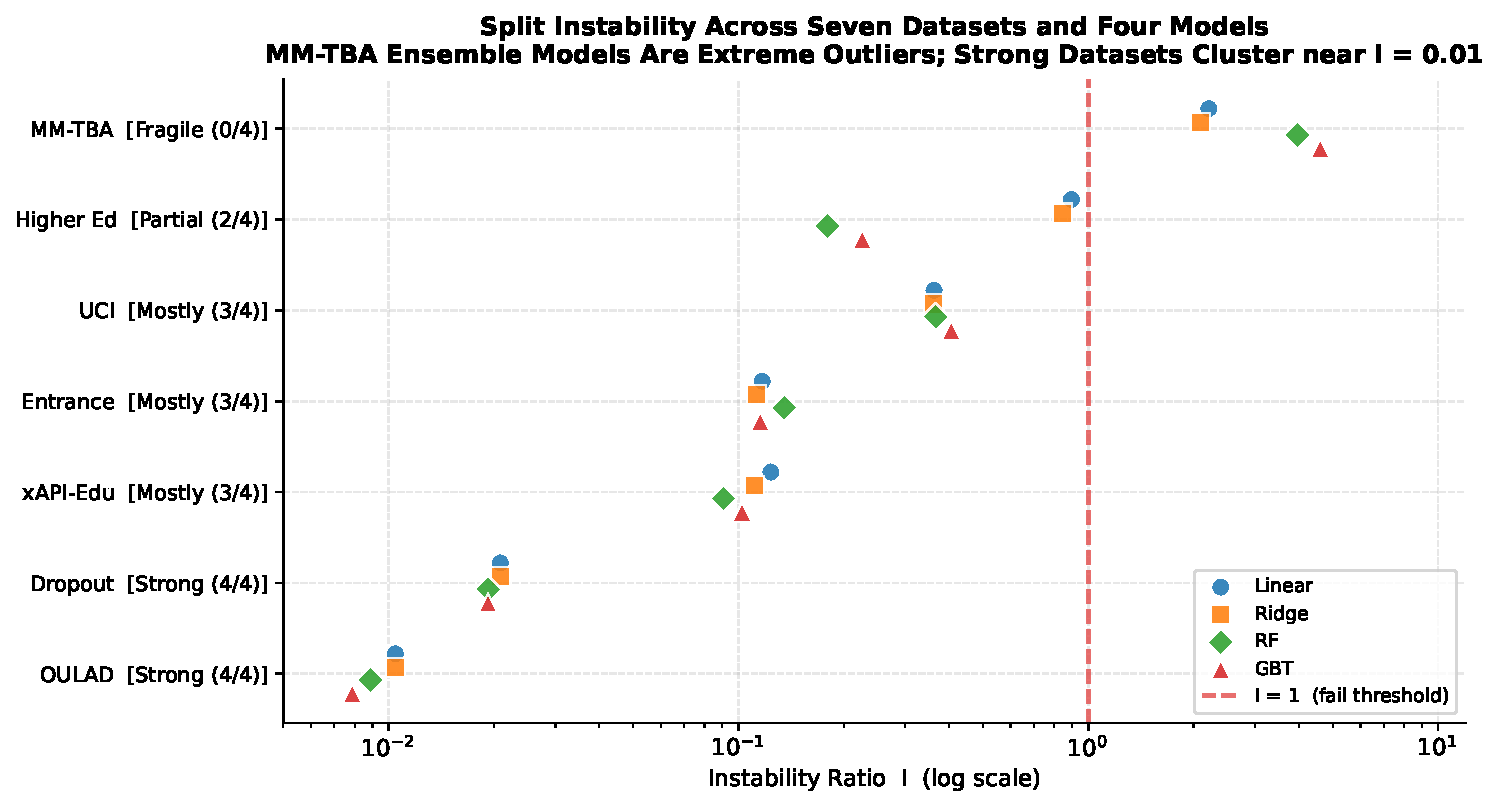
\includegraphics[width=0.95\textwidth]{fig5_instability_strip.pdf}
\caption{Instability ratio ($I$) for all seven datasets and four models (log scale). The dashed red line marks $I = 1$, the failure threshold where between-split variance equals the mean advantage over baseline. MM-TBA's Gradient Boosting ($I = 4.6$) and Random Forest ($I = 4.0$) are extreme outliers; structurally sound datasets (OULAD, Dropout) cluster near $I = 0.01$.}
\label{fig:instability_strip}
\end{figure}

\subsection{Classification-Metric Sensitivity Check}

To verify that the regression-framing audit conclusions are not an artifact of metric choice, the four datasets with binary or ordinal targets were re-evaluated under classification-appropriate metrics (Table 4).

\begin{table*}[htbp]
\centering
\caption{Classification-metric sensitivity check on the four datasets with binary or ordinal targets. Accuracy and AUC-ROC are reported for each classifier under iid 100-split resampling and group-aware holdout. $I_{\mathrm{acc}}$ is the accuracy-based instability ratio.}
\label{tab:classification_sensitivity}
\resizebox{\textwidth}{!}{%
\begin{tabular}{l l c c c c c}
\toprule
Dataset & Classifier & iid Acc (mean $\pm$ SD) & iid AUC & $I_{\mathrm{acc}}$ & Group Acc (mean) & Group AUC \\
\midrule
OULAD & Logistic & $0.837 \pm 0.004$ & $0.910$ & $0.013$ & $0.817$ & $0.920$ \\
(binary) & RF & $0.849 \pm 0.004$ & $0.922$ & $0.012$ & $0.825$ & $0.926$ \\
 & GBT & $0.861 \pm 0.004$ & $0.938$ & $0.011$ & $0.842$ & $0.939$ \\
\midrule
Dropout & Logistic & $0.912 \pm 0.009$ & $0.953$ & $0.031$ & $0.897$ & $0.943$ \\
(binary) & RF & $0.907 \pm 0.010$ & $0.952$ & $0.035$ & $0.885$ & $0.928$ \\
 & GBT & $0.909 \pm 0.010$ & $0.954$ & $0.033$ & $0.886$ & $0.938$ \\
\midrule
xAPI-Edu & Logistic & $0.737 \pm 0.038$ & $0.870$ & $0.131$ & $0.702$ & $0.866$ \\
(3-class) & RF & $0.795 \pm 0.035$ & $0.916$ & $0.102$ & $0.750$ & $0.895$ \\
 & GBT & $0.758 \pm 0.043$ & $0.883$ & $0.141$ & $0.694$ & $0.861$ \\
\midrule
Entrance Exam & Logistic & $0.511 \pm 0.039$ & $0.761$ & $0.191$ & $0.420$ & $0.695$ \\
(4-class) & RF & $0.487 \pm 0.038$ & $0.725$ & $0.207$ & $0.402$ & $0.686$ \\
 & GBT & $0.502 \pm 0.040$ & $0.749$ & $0.203$ & $0.458$ & $0.748$ \\
\bottomrule
\end{tabular}}%
\end{table*}

Classification-metric results confirm the regression-framing conclusions (Table 4). OULAD and Dropout retain Strong profiles (iid accuracy 0.84--0.91, $I_{\mathrm{acc}} \leq 0.035$, group-holdout AUC $> 0.92$). xAPI-Edu remains Mostly Passing (RF group-holdout accuracy 75.0\%, AUC $= 0.895$). Entrance Exam shows the weakest performance (Logistic iid accuracy 51.1\% on a 4-class task with majority baseline 30.5\%, group-holdout AUC $= 0.69$--$0.75$), consistent with the regression-framing assessment of moderate but fragile signal; the low absolute accuracy partly reflects the inherent difficulty of 4-class ordinal prediction.

\FloatBarrier
\clearpage
\section{Discussion}

The seven-dataset audit reveals three systemic findings about the state of educational prediction benchmarks.

\textbf{Finding 1: Group-level confounding is pervasive but graded.} Five of seven educational datasets fail linear-model group-aware holdout, decomposing into two categories. Three exhibit \textbf{model-invariant} confounding: UCI Student ($R^2 \approx 0.00$ even for RF/GBT), Higher Ed ($R^2 < -8$ for all models), and MM-TBA (untestable but failing all other dimensions). Two exhibit \textbf{remediable linear-specific} overfitting: xAPI-Edu (ridge $R^2 = 0.50$, RF $R^2 = 0.58$ under group holdout) and Entrance Exam (RF $R^2 = 0.33$). This distinction matters for practitioners: xAPI-Edu's failure is largely remediable through regularization, while UCI Student's persists even for ensemble models, indicating genuine school-level confounding.

\textbf{Finding 2: Fragility is algorithm-invariant.} On MM-TBA, upgrading from linear regression ($I = 2.2$) to Gradient Boosting ($I = 4.6$) doubles the instability. On Higher Ed, RF improves iid $R^2$ from 0.04 to 0.52 but collapses equally under group holdout ($R^2 = -13.0$). On structurally sound datasets, ensemble models yield genuine gains without introducing instability (see Fig~\ref{fig:instability_strip}).

\textbf{Finding 3: The audit protocol discriminates meaningful quality gradients.} The seven datasets span a structured continuum from Fragile (0/4) through Partial (2/4) and Mostly Passing (3/4) to Strong (4/4). This gradient should be interpreted cautiously: it partly reflects sample size ($N = 145$ to $32{,}593$) and feature-target proximity. OULAD's strong profile is partly expected because its behavioral-performance features (assessment scores, VLE clicks) are definitionally close to the binary pass/fail outcome. An instructive contrast is UCI Student vs. xAPI-Edu: despite similar sample sizes ($N = 649$ vs. $480$) and comparable iid $R^2$ ($0.26$ vs. $0.60$), they diverge sharply under group holdout---UCI collapses to $R^2 \approx 0.00$ even for ensemble models, while xAPI-Edu recovers to $R^2 = 0.58$ with RF. The divergence traces to the nature of the grouping structure: UCI's 2 schools (GP: $n=423$; MS: $n=226$) represent distinct institutional contexts with large distributional gaps, whereas xAPI-Edu's 12 topics share a common platform and student population. With only 2 groups, UCI's leave-one-group-out holdout effectively trains on one school and tests on another, making the evaluation maximally sensitive to between-group heterogeneity. This illustrates that group-holdout severity depends on both the number and heterogeneity of groups, not merely on sample size. Nevertheless, the practical value lies in the specific failure mechanisms identified: each profile level corresponds to a different remediation pathway. Fragile datasets (MM-TBA) require fundamental data-quality improvement. Partial datasets (Higher Ed) need larger samples and broader group coverage. Mostly Passing datasets (xAPI-Edu, Entrance Exam, UCI) may benefit from regularization-aware evaluation protocols or supplementary group-aware analysis. Strong datasets (OULAD, Dropout) support cautious benchmark claims.

Taken together, these three findings sharpen the paper's contribution in three concrete ways.

(1) \textbf{The audit findings carry direct socio-technical implications for educational deployment. } The UCI school-level confounding means a model deployed across schools could systematically mispredict outcomes. The MM-TBA instability means the same teacher could be rated differently depending on which random split was used. The audit thus serves as a minimum-viable quality gate before educational prediction models influence decisions about teachers or students.

(2) \textbf{These dimensions also connect the audit protocol to established educational measurement theory. } The instability ratio $I$ operationalizes a concern central to Generalizability Theory \citep{Brennan2001}: when $I \geq 1$, the benchmark conclusion is not generalizable across train-test partitioning. The group-holdout dimension operationalizes a Messick~\citep{Messick1995}-style validity requirement: a dataset whose signal collapses under group-aware evaluation lacks generalizability evidence. An important caveat is that group-holdout collapse does not uniquely diagnose confounding; it may also reflect legitimate distributional shift. Distinguishing the two requires domain knowledge that the audit flags the need for but does not itself provide. As a practical heuristic, the following diagnostic sequence is suggested. When all model types collapse under group holdout (as with UCI Student and Higher Ed), the first step is to compare group-level feature distributions---large distributional gaps between groups point toward genuine cross-context heterogeneity rather than statistical confounding. When only unregularized linear models collapse while ridge or ensemble models recover (as with xAPI-Edu), overfitting on high-dimensional features is the more parsimonious explanation, and regularization may suffice. When group counts are very small ($k \leq 3$), leave-one-group-out holdout inherently functions as cross-distribution extrapolation, and results should be interpreted as stress tests of out-of-distribution robustness rather than direct evidence of latent confounders.

(3) \textbf{A persistent practice gap motivates the broader adoption of such diagnostics.} Educational prediction papers rarely report split-instability diagnostics, permutation nulls, or group-aware holdout results. The present study demonstrates that systematic application of existing diagnostics reveals evaluation fragility that headline metrics conceal. It is worth noting that related frameworks---Model Cards \citep{Mitchell2019} and Dataset Nutrition Labels \citep{Holland2020}---address complementary concerns; the present protocol adds a computational stress-test layer.

\section{Limitations}

The seven-dataset gradient should not be over-interpreted as evidence that the audit procedure has inherent discriminative calibration, because it is partly confounded with sample size, feature-target proximity, and task-construct differences. The operational thresholds ($I \geq 1$, group-holdout $R^2$ retention $\geq 50\%$) are empirically motivated but not yet calibrated across a large benchmark corpus. For example, Higher Ed's linear-model beat rate of 0.83 places it in the borderline zone between pass (0.90) and fail (0.80): at a pass threshold of 0.80 it would pass baseline gap, at 0.90 it fails. Similarly, a 40\% (rather than 50\%) group-holdout retention threshold would not change any current assignment but could affect future datasets near the boundary. Until the thresholds are calibrated on a larger benchmark corpus, practitioners should treat them as informed defaults rather than universal cutoffs.

The permutation-null dimension is estimated on only 10 of 100 splits per dataset, yielding Perm\% estimates with wide binomial uncertainty: 95\% Clopper--Pearson CIs span [0.03, 0.56] for Perm\% $= 0.20$ (MM-TBA) and [0.44, 0.97] for Perm\% $= 0.80$ (Higher Ed). This uncertainty does not affect the two extreme values (Perm\% $= 1.00$ for five datasets, CI [0.69, 1.00]), but borderline cases should be interpreted with the confidence intervals in mind. Expanding the permutation analysis to 30--50 splits per dataset would narrow these intervals and is recommended for future applications of the protocol.

The group-holdout results are sensitive to the number and size of groups: UCI has only 2 schools, Entrance Exam has 3 boards, while Dropout has 17 programs---making cross-dataset comparisons of group-holdout severity approximate. The four audit dimensions are currently given equal weight in assigning profile labels (Fragile through Strong); in practice, domain context may warrant differential emphasis---for example, metadata adequacy may be more consequential than split instability for high-stakes deployment decisions.

All seven datasets are from European, Portuguese, Jordanian, Indian, or Chinese educational contexts; generalization to other settings remains untested. The audit uses linear baselines and two ensemble methods; other model families (e.g., deep learning) might yield different instability patterns on some datasets, though the algorithm-invariance finding across four model types suggests this is unlikely to change the main conclusions. A stronger next-stage study should include datasets with richer grouping metadata (e.g., teacher-level or classroom-level identifiers) and, where available, paired evidence on agreement between automated and human scoring.

\section{Conclusion}

This study proposes and validates a four-dimension pre-modeling audit protocol for educational prediction benchmarks and applies it to seven public datasets. The main findings are:

(1) \textbf{Pervasive group-level confounding.} Five of seven datasets fail linear-model group-aware holdout. Two exhibit confirmed model-invariant confounding with empirical group-holdout evidence (UCI Student, Higher Ed), two show remediable linear-specific overfitting (xAPI-Edu, Entrance Exam), and one (MM-TBA) fails all other dimensions but cannot be tested for group-holdout collapse because grouping metadata is unavailable.

(2) \textbf{Algorithm-invariant fragility.} Ensemble models amplify instability on fragile data ($I \approx 4.6$ vs. $2.2$ on MM-TBA) and yield genuine gains only on structurally sound data.

(3) \textbf{Structured quality gradient.} The audit assigns profiles from Fragile (0/4) to Strong (4/4), with each level corresponding to different remediation needs.

(4) \textbf{Model-dependent group holdout.} Regularized and ensemble models sometimes survive group holdout where linear regression collapses, indicating that metadata adequacy should be evaluated jointly with model capacity.

(5) \textbf{Metric robustness.} A classification-metric sensitivity check confirms that audit profiles are robust to metric choice.

Based on these empirical patterns, the following operational decision criteria are proposed:

\begin{table}[htbp]
\centering
\caption{Operational decision criteria derived from the seven-dataset audit. Thresholds are empirically motivated and intended as practical starting points.}
\label{tab:decision_criteria}
\resizebox{\textwidth}{!}{%
\begin{tabular}{p{2.5cm} p{2.8cm} p{2.5cm} p{4.5cm}}
\toprule
Audit dimension & Pass criterion & Fail indicator & Recommended action on failure \\
\midrule
Baseline gap & $\Delta_{\mathrm{MAE}} > 0$ with beat rate $\geq 0.90$ across $\geq 50$ splits & Beat rate $< 0.80$ or $\Delta_{\mathrm{MAE}}$ smaller than cross-split SD & Do not escalate to complex models; investigate target quality and feature relevance \\

Split instability & $I < 1.0$ (model variability smaller than gain) & $I \geq 1.0$ & Increase sample size, reduce feature dimensionality, or improve split design \\

Null separation & Permutation $p < 0.05$ consistent across $\geq 80\%$ of splits & Inconsistent or non-significant separation & Treat as insufficient evidence; do not publish benchmark claims \\

Metadata adequacy & Group holdout retains $\geq 50\%$ of iid $R^2$ under the linear reference model & $R^2$ collapse under group holdout & Add grouping metadata; run group-aware validation before deployment \\
\bottomrule
\end{tabular}}%
\end{table}

For reuse, the procedure is summarized as a four-step audit checklist:

(1) \textbf{Verify baseline gap}: does the proposed predictor beat a trivial baseline by a margin that is practically meaningful and reproducible across resampled splits?

(2) \textbf{Stress-test split instability}: does between-split variability remain smaller than the reported gain ($I < 1$)?

(3) \textbf{Check null separation}: are permutation-based significance tests consistent across admissible splits?

(4) \textbf{Audit metadata adequacy}: does performance survive group-aware holdout, and are the provenance fields needed for leakage-resistant validation present in the release?

If all four checks pass, the dataset supports cautious benchmark claims. If one or two fail, targeted remediation may be sufficient. If three or more fail, the dataset is better treated as a research-stage resource requiring substantial revision before benchmark conclusions are drawn.

\section*{Author Contributions}
Conceptualization, Y.M. and L.Z.; methodology, Y.M. and L.Z.; software, L.Z.;
validation, Y.M. and L.Z.; formal analysis, Y.M.; investigation, Y.M.; data curation,
Y.M. and L.Z.; visualization, L.Z.; writing---original draft preparation, Y.M.;
writing---review and editing, Y.M. and L.Z.; supervision, L.Z. All authors have
read and agreed to the published version of the manuscript.

\section*{Funding}
This study was funded by the Education Department of Hunan Province, China.
Project Name: Empirical Study on the Impact of Changes in College English Classroom
Environment on Students' Engagement, Project Number: HNJG-2022-0608.

\section*{Institutional Review}
According to the institutional policy governing secondary analysis of existing public
datasets at Hunan Agricultural University, ethical review and approval were waived for
this study because it used existing public dataset releases, involved no direct
interaction with human participants, and analyzed no newly collected personal data.

\section*{Data Availability}
All seven datasets are publicly available from their original maintainers. The audit
protocol implementation and analysis scripts are available at
\url{https://github.com/zhanglizhuo/BehaviorAudit}.

\section*{Acknowledgments}
The authors thank the teams behind the seven audited datasets for their commitment
to open data.

\section*{Conflicts of Interest}
The authors declare no conflicts of interest.

\section*{Abbreviations}
\noindent
\begin{tabular}{@{}ll}
MM-TBA & Multi-Modal Dataset for Teacher Behavior Analysis \\
OULAD  & Open University Learning Analytics Dataset \\
MAE    & Mean Absolute Error \\
EDM    & Educational Data Mining \\
RF     & Random Forest \\
GBT    & Gradient Boosting \\
\end{tabular}

\nolinenumbers

\bibliography{behavioraudit}

\end{document}
